\section{Temperature}

\begin{multicols}{2}


\subsection{Principle of a Thermometer}

\begin{center}
\includegraphics[width=0.4\textwidth]{./img/source/thermometer.png}
\end{center}

\begin{description*}
%\item[Subtopic:]{}
\item[Materials:]{Bottle, pen tube, stopper/cork/rubber cylinder, food colouring, hot water bath}
%\item[Setup:]{}
\item[Procedure:]{Fill a bottle (about 500 mL) with coloured water up to the rim. Tightly fix a stopper carrying a narrow pen tube into the mouth of the bottle. The liquid level should be just visible above the stopper. Now place the bottle into hot water and heat it for a short time.}
%\item[Hazards:]{}
\item[Observations:]{The liquid level rises after heating.}
\item[Theory:]{When liquids are heated, they expand. A thermometer can be made by calibrating the change in volume according to temperature change for a given liquid.}
\item[Applications:]{Clinical thermometers use mercury, while many outdoor thermometers use alcohol. The expansion of alcohol is six times greater than that of mercury. Mercury has a higher boiling point, so it is used to measure higher temperatures.}
\item[Questions:]{Why is water typically not used in thermometers?}
%\item[Notes:]{}
\end{description*}

\vfill
\columnbreak

\subsection[Fixed Points of a Thermometer]{Fixed Points of a \hfill \\ Thermometer}

\begin{center}
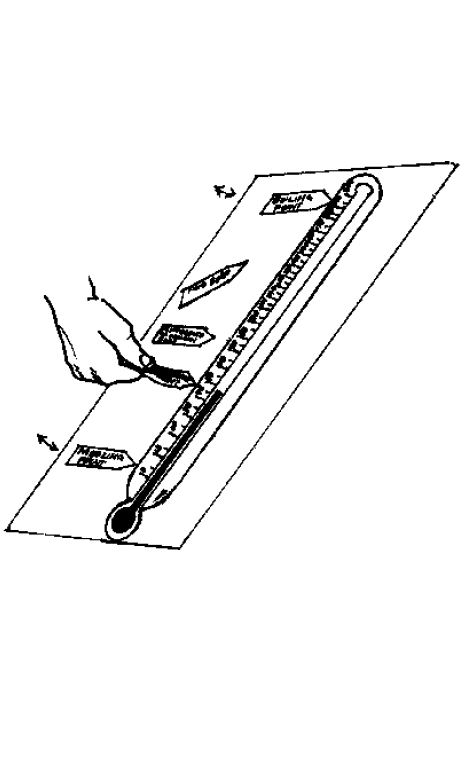
\includegraphics[width=0.4\textwidth]{./img/source/fixed-points.png}
\end{center}

\begin{description*}
%\item[Subtopic:]{}
\item[Materials:]{Cardboard/manila paper, tape, marker pens}
%\item[Setup:]{}
\item[Procedure:]{Draw a large diagram or display chart of a thermometer on manila paper. Use coloured arrows to indicate the characteristic fixed points for water and other substances. Make separate charts for the Fahrenheit, Centigrade and Kelvin scales.}
%\item[Hazards:]{}
%\item[Questions:]{}
%\item[Observations:]{}
%\item[Theory:]{}
%\item[Applications:]{}
%\item[Notes:]{}
\end{description*}

\vfill
\pagebreak

%==================================================================================================%




\end{multicols}

%\pagebreak